\section{Der Algorithmus}

\subsection{Hauptablauf Algorithmus}
Zu Beginn wird ein Simplex gebildet, indem f�r jede Ecke i des Simplex ein $x_i$ ausgew�hlt wird. 
Mit den gew�hlten $x_i$ werden nun die dazu geh�rigen $y_i$ der Zielfunktion ausgerechnet. \\
Aus den erhaltenen Funktionswerten wird der beste $y_{min}$ sowie der schlechteste $y_{max}$ betrachtet. Wenn der beste Wert gut genug ist, dann ist der Algorithmus schon fertig, bevor er eigentlich begonnen hat. Es ist nat�rlich eher Zufall, wenn man gleich bei der ersten Wahl des Simplex das Minima trifft, meistens hat man es nicht getroffen und muss nun auf Grund des gew�hlten Simplex ein neues Simplex bilden. 

\resizebox{1\textwidth}{!}{
\providecommand{\highlight}{white}
\begin{tikzpicture}[node distance = 1.7cm,every node/.style={rectangle,fill=white},
  block/.style={draw,align=center},
  highlight/.style={draw,fill=\highlight},
  line/.style = {draw,-latex'}
]

\node (start) [block] {N+1 Startpunkte $x_i$ w"ahlen (Simplex bilden)};

\node (a1) [block, below of=start] { $y_i = f(x_i)$ berechnen};

\node (a2) [block, below of=a1] { Bestes ($y_{min}$) und schlechtestes ($y_{max}$) $y_i$ bestimmen};

\node (a3) [block, below of=a2,text width=5cm]{Abbruchbedingung erf"ullt?};

\node (ende) [block, below of=a3] {Ende};

\node (a4) [highlight, left of=a3, node distance=6cm] {Neuer Simplex bilden};



\path[line] (start) -- (a1);
\path[line] (a1) -> (a2);
\path[line] (a2) -> (a3);

\path[line] (a3) -> node{ja} (ende);
\path[line] (a3) -> node{nein} (a4);

\path[line] (a4)  |-  (a1.west);

\end{tikzpicture}
}


\subsection{Auswahlverfahren neues Simplex}
Das Auswahlverfahren des neuen Simplex unterliegt eine Reihe von Entscheidungen auf Grund der gegebenen Eckpunkte sowie deren Funktionswerte. Auf Seite XXX findet man diesen Entscheidungsbaum.\\
Wenn man das Diagramm etwas genauer betrachtet, f�llt einem auf, dass zu Beginn das Simplex ziemlich grob behandelt wird, indem man erst einmal durch Reflexion versucht, weg vom schlechtesten Punkt zu kommen. War diese Entscheidung erfolgreich wird auch noch gleich in die neue Richtung gestreckt, um das Simplex in die vermeintlich richtige Richtung zu treiben. \\
Erst wenn diese Methode nicht funktioniert hat, wird etwas detaillierter auf das Simplex und seine Position eingegangen, indem man beispielsweise schaut, ob der reflektierte Funktionswert zumindest besser ist als der zweitschlechteste. \\
Methoden wie die Kontraktion oder auch die Komprimierung sind dann schliesslich eher Feineinstellungen, man versucht etwas n�her zum Schwerpunkt zu r�cken, um zu schauen, wie sich die neuen Eckpunkte in der Zielfunktion verhalten.\\
Das ganze ist nat�rlich sehr abh�ngig von dem zu Beginn gew�hlten Simplex. Der Algorithmus findet - bis auf wenige Ausnahmen - immer ein Minima. Wenn er jedoch st�ndig in ein lokales Minima f�llt, muss man sich vielleicht �berlegeben die Startbedingungen zu �ndern, indem man das Simplex beispielsweise �ber ein gr�sseres Gebiet aufspannt.\\
\usetikzlibrary{shapes}
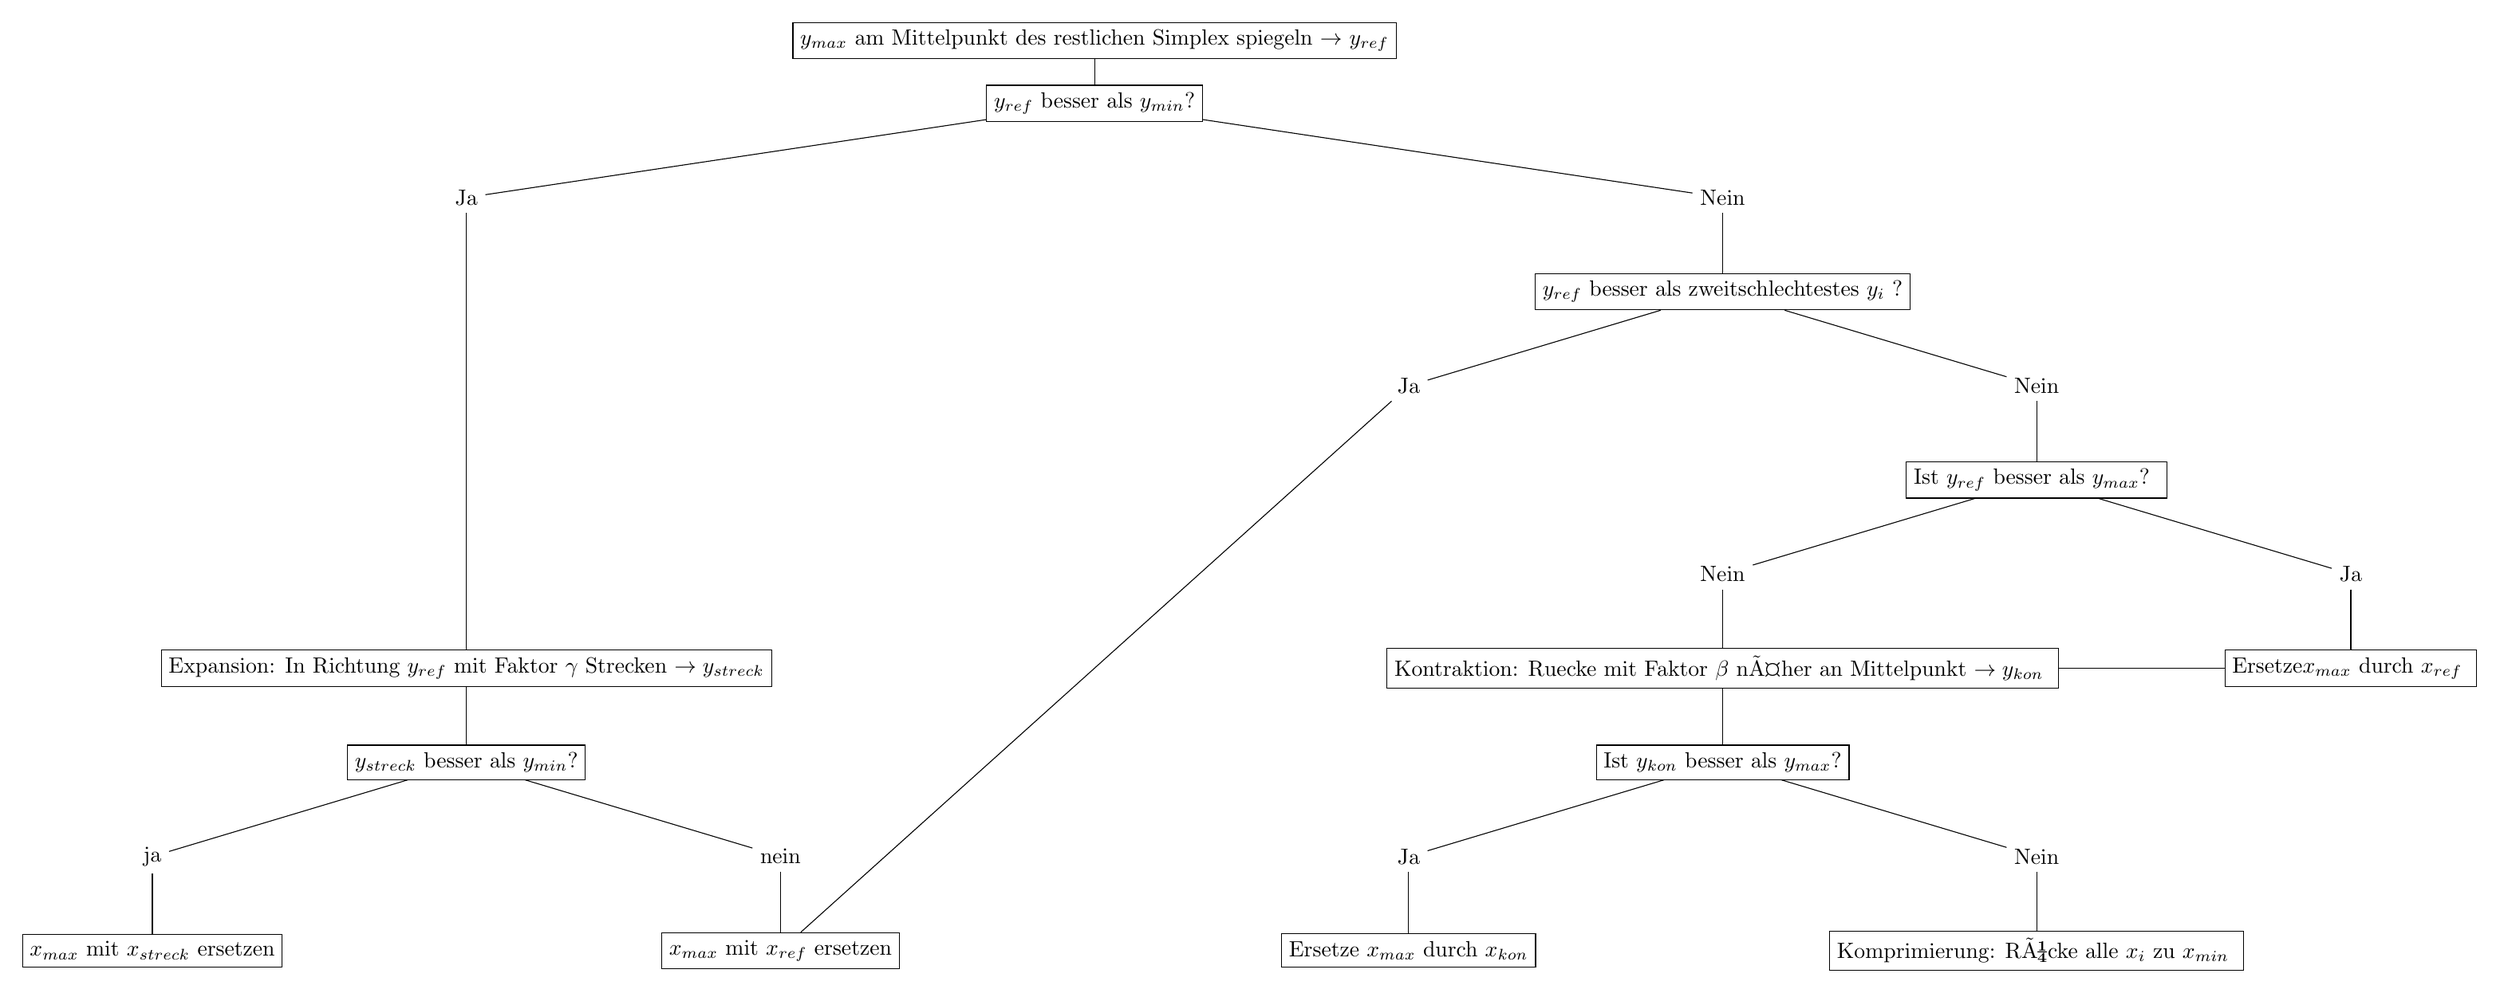
\begin{tikzpicture}[
  top/.style={draw,align=center},
  med/.style={draw,align=center},
  fin/.style={ellipse,draw,align=center}
]

\tikzstyle{level 1}=[sibling distance=200mm,align=center]
\tikzstyle{level 2}=[sibling distance=100mm,align=center]
%\tikzstyle{level 3}=[sibling distance=100mm]


\node (start) at (0,1)[draw] {$y_{max}$ am Mittelpunkt des restlichen Simplex spiegeln $\rightarrow$ $y_{ref}$};

\node[top](top){$y_{ref}$ besser als  $y_{min}$?}
	child { node {Ja} child {child { child  { child { child {
		node[med] {Expansion: In Richtung $y_{ref}$ mit Faktor $\gamma$ Strecken  $\rightarrow y_{streck} $}
		child{
			node[med]  {$y_{streck}$ besser als $y_{min}$?}
			child { node {ja}
			child { node [med]{$x_{max}$ mit $x_{streck}$ ersetzen} }}
			child { node {nein}
			child { node(a2) [med]{$x_{max}$ mit $x_{ref}$ ersetzen} }}
		}
	}}}}}}
	child {
		node {Nein}
		child  {
		node [med] {$y_{ref}$ besser als zweitschlechtestes $y_i$ ?}
		child { node (b1) [] {Ja} }
		child { node {Nein} 
		child { node[med] {Ist $y_{ref}$ besser als $y_{max}$? }
			child {node{Nein}
				child { node (kont)[med] {Kontraktion: Ruecke mit Faktor $\beta$ näher an Mittelpunkt $\rightarrow y_{kon}$ }
					child { node[med]  {Ist $y_{kon}$ besser als $y_{max}$?}
						child {node {Ja}
							child {node[med] {Ersetze $x_{max}$ durch $x_{kon}$}}
						}
						child {node {Nein}
							child {node[med] {Komprimierung:  Rücke alle $x_i$ zu $x_{min}$ } }
						}
					}
				}
			}
			child {node {Ja}
				child { node (zukont)[med] {Ersetze$ x_{max}$ durch $x_{ref}$ } }
			}
		}
		}
	}
	}
;
\draw (zukont) -- (kont);
\draw (b1) -- (a2);
\draw (start) --(top);

\end{tikzpicture}


\subsection{Probleme des Verfahrens}
